\documentclass[11pt,a4paper]{article}
\usepackage[margin=1in]{geometry}
\usepackage[T1]{fontenc}
\usepackage[utf8]{inputenc}
\usepackage{lmodern}
\usepackage{microtype}
\usepackage{graphicx}
\graphicspath{{figures/}}
\usepackage{amsmath}
\usepackage{amssymb}
\usepackage{hyperref}
\usepackage{parskip}
\usepackage{enumitem}
\usepackage{booktabs}

\hypersetup{
    colorlinks=true,
    linkcolor=blue,
    urlcolor=blue,
    pdftitle={A Reader's Guide to Information Geometry of the Quantum-Classical Boundary},
    pdfauthor={Ian Todd}
}

\title{\textbf{A Reader's Guide to\\Information Geometry of the Quantum-Classical\\Boundary in Biological Information Processing}}
\author{Ian Todd}
\date{Companion note for the manuscript submitted to \emph{BioSystems}}

\begin{document}

\maketitle

\section*{Who this is for}

This note is for readers who want to understand what the paper proves without working through the full manuscript of theorems and Lindblad dynamics.  It assumes you are comfortable with science writing and know roughly what a quantum state is, but not that you have met information geometry or quantum biology before.  Every technical term is explained when it first appears.

It is not a substitute for the paper.  It is a map: what question the paper asks, what it proves, what is genuinely new, and what remains open.

\section*{The one-sentence claim}

\textbf{Decoherence---the process by which quantum systems become classical---is a structured geometric projection from a higher-dimensional quantum state space onto a lower-dimensional classical one, and the geometry of this collapse determines what biology can exploit.}

That statement has four parts:
\begin{enumerate}[leftmargin=1.5em]
\item quantum states have more distinguishable directions than classical probability distributions;
\item dephasing removes exactly the directions associated with quantum coherence;
\item the geometry of the surviving classical directions can be quantified precisely;
\item photosynthetic complexes operate at dephasing rates where this geometry is nearly classical.
\end{enumerate}

\section*{Background: what you need to know}

\subsection*{Quantum states and density matrices}

A quantum system with $d$ energy levels is described by a \emph{density matrix}~$\rho$: a $d \times d$ matrix that is positive (all eigenvalues non-negative) and has trace~1.  The diagonal entries are the \emph{populations}---the probabilities of finding the system in each energy level.  The off-diagonal entries are the \emph{coherences}---they encode phase relationships between energy levels and are responsible for interference effects.

A \emph{classical} probability distribution is just the diagonal: $d$ non-negative numbers summing to~1.

\subsection*{Degrees of freedom}

A $d \times d$ density matrix has $d^2 - 1$ independent real parameters.  Of these, $d - 1$ are populations and $d^2 - d$ are coherences.  For a 7-site photosynthetic complex: 48 total parameters, 6 populations, 42 coherences.

Dephasing eliminates the $d^2 - d$ coherence parameters and preserves the $d - 1$ population parameters.  That is the dimensional collapse:
\[
d^2 - 1 \;\longrightarrow\; d - 1.
\]

\subsection*{Metrics: measuring distances between states}

To make ``geometry'' precise, we need a way to measure distances between quantum states.

The \textbf{Bures metric} is the standard distance measure on quantum states.  It measures how statistically distinguishable two nearby states are: if two states are hard to tell apart by any measurement, their Bures distance is small.

The \textbf{Fisher--Rao metric} is the analogous measure on classical probability distributions.

A key fact: when you restrict the Bures metric to diagonal states, you recover the Fisher--Rao metric exactly.  So the classical metric lives naturally inside the quantum metric.

\subsection*{Tangent spaces and orthogonality}

At any state~$\rho$, the \emph{tangent space} splits into:
\begin{itemize}[leftmargin=1.5em]
\item \emph{population directions}: changes to the diagonal entries;
\item \emph{coherence directions}: changes to the off-diagonal entries.
\end{itemize}

The paper asks: are these two sets of directions \emph{perpendicular} (orthogonal) under the Bures metric?  If they are, classical and quantum information are geometrically independent.  If not, the two types of information are entangled in the metric.

\section*{The basic picture}

\begin{figure}[ht]
\centering
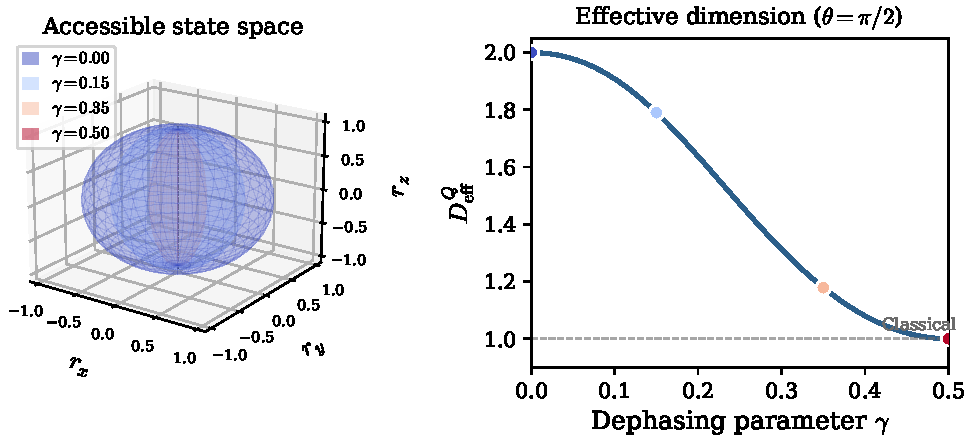
\includegraphics[width=0.92\textwidth]{fig1_bloch_collapse.pdf}
\caption{Dephasing removes coherence directions and leaves the classical simplex.  For a qubit, the full quantum state space is the 3-dimensional Bloch ball; dephasing collapses it onto the 1-dimensional $z$-axis.}
\end{figure}

The paper uses \emph{dimensional collapse} because dephasing does not blur the state randomly---it projects it onto a specific, lower-dimensional subspace.  The dimensions lost are precisely the coherence directions.

\section*{The main mathematical results}

\subsection*{Result 1: Exact qubit angle (Theorem 3.4)}

At diagonal states, the population and coherence directions are perfectly perpendicular ($90^\circ$) under the Bures metric.

Away from the diagonal, the separation becomes oblique.  For qubits, the paper proves:
\[
\cos^2 \theta_B
=
\frac{r_z^2\, r_\perp^2}{(1-r_\perp^2)(1-r_z^2)},
\]
where $r_z$ is the population imbalance and $r_\perp$ the coherence magnitude.

This says:
\begin{itemize}[leftmargin=1.5em]
\item the split is perpendicular ($\theta_B = 90^\circ$) when the state is diagonal ($r_\perp = 0$);
\item it is also perpendicular when populations are equal ($r_z = 0$), even with coherence;
\item under dephasing ($r_\perp$ shrinking), the angle moves back toward $90^\circ$.
\end{itemize}

\textbf{Key point:} as decoherence proceeds, the classical/quantum split sharpens.

\begin{figure}[ht]
\centering
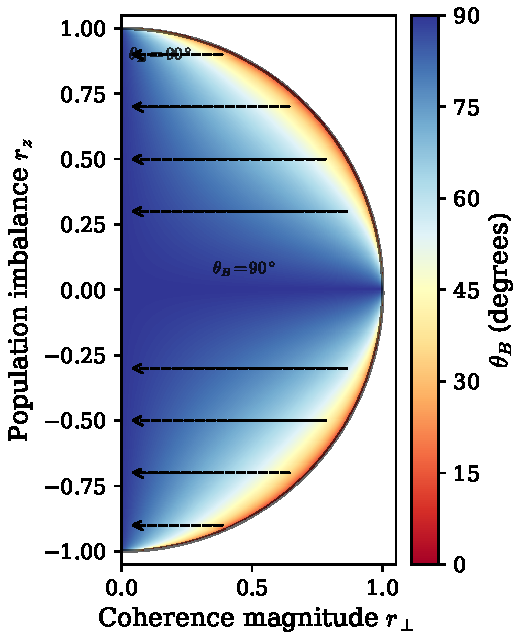
\includegraphics[width=0.92\textwidth]{fig3_bures_angle.pdf}
\caption{The Bures angle across the Bloch ball.  Orthogonality ($90^\circ$) holds along the $z$-axis (diagonal states) and the equatorial plane (equal populations).  The angle drops below $90^\circ$ only where both coherence and population imbalance are nonzero.}
\end{figure}

\subsection*{Result 2: Global orthogonality theorem (Theorem 3.6)}

For $d \geq 3$, the paper proves the complete statement: the population and coherence tangent subspaces are Bures-orthogonal \textbf{if and only if} $\rho$ is diagonal.  Any coherence breaks the clean classical--quantum split.

This is stronger than the qubit case, where equal populations can preserve orthogonality even with coherence.

\subsection*{Result 3: Perturbative cross-Gram formula (Theorem 3.7)}

Near the classical simplex (small coherences), the paper gives an explicit formula for how much orthogonality is broken.  The cross-Gram entries between population and coherence directions are linear in coherence at leading order, so even small coherences produce a measurable departure from orthogonality.

\section*{The biological application}

\subsection*{Environment-assisted quantum transport (ENAQT)}

Photosynthetic complexes transfer absorbed light energy from antenna pigments to a low-energy acceptor (a reaction centre in some complexes, a ``red pool'' of terminal chromophores in others).  In 2008--2009, several groups discovered that \emph{intermediate} dephasing enhances transport efficiency: too little dephasing and quantum interference creates destructive trapping; too much and the quantum speedup is lost.  The optimal intermediate regime is called ENAQT.

The paper asks: \textbf{what does state space look like at the ENAQT optimum?}

\subsection*{FMO complex ($d = 7$)}

The Fenna--Matthews--Olson complex from green sulfur bacteria has 7 bacteriochlorophyll sites.

\begin{itemize}[leftmargin=1.5em]
\item \textbf{Collapse:} $d^2 - 1 = 48$ quantum dimensions $\to$ $d - 1 = 6$ classical dimensions.
\item \textbf{ENAQT peak:} Transport efficiency maximized at $\gamma_{\mathrm{opt}} \approx 100$--$150\;\mathrm{cm}^{-1}$.
\item \textbf{Geometry at optimum:} All 6 Bures principal angles exceed $87^\circ$.  The state is geometrically almost classical.
\item \textbf{Strong mixing regime:} Principal angles drop significantly only at $\gamma \lesssim 10\;\mathrm{cm}^{-1}$, well below the biological operating point.
\end{itemize}

\begin{figure}[ht]
\centering
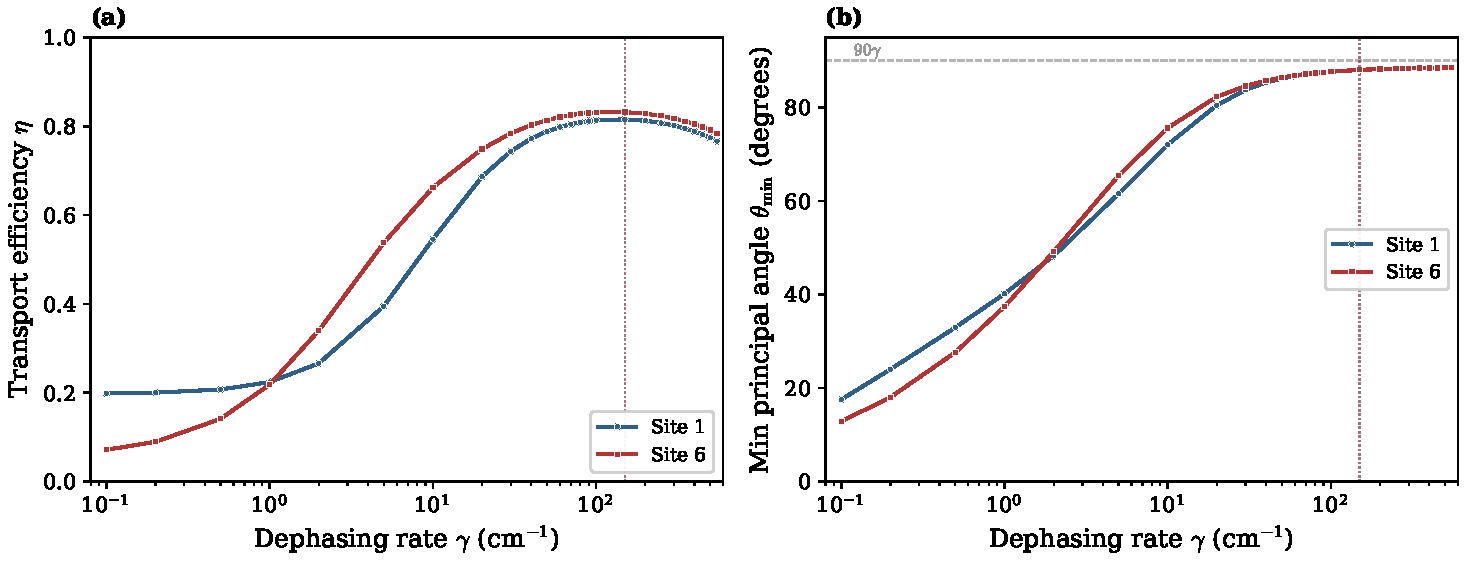
\includegraphics[width=0.92\textwidth]{fig4_fmo_collapse.pdf}
\caption{FMO results. (a)~Transport efficiency versus dephasing rate. (b)~The six Bures principal angles: all above $87^\circ$ at the ENAQT optimum, indicating near-classical geometry.}
\end{figure}

\subsection*{PE545 antenna complex ($d = 8$)}

To test whether the FMO result is specific to one complex, the paper applies the same analysis to PE545 from the cryptophyte alga \emph{Rhodomonas} CS24.  PE545 differs from FMO in every structural detail: 8 bilin chromophores (not bacteriochlorophylls), C$_2$ pseudo-symmetry, a central dimer as energy input (not peripheral injection), and energy transfer to a low-energy acceptor manifold (not a single reaction centre).

\begin{itemize}[leftmargin=1.5em]
\item \textbf{Collapse:} $63 \to 7$ dimensions.
\item \textbf{Optimal dephasing:} $\gamma_{\mathrm{opt}} \approx 700$--$750\;\mathrm{cm}^{-1}$ (higher than FMO due to larger site-energy disorder).
\item \textbf{Geometry at optimum:} All 7 principal angles exceed $89^\circ$---even more classical than FMO.
\item \textbf{Robustness:} The result survives changes to the target manifold definition and halving the trapping rate.
\end{itemize}

\begin{figure}[ht]
\centering
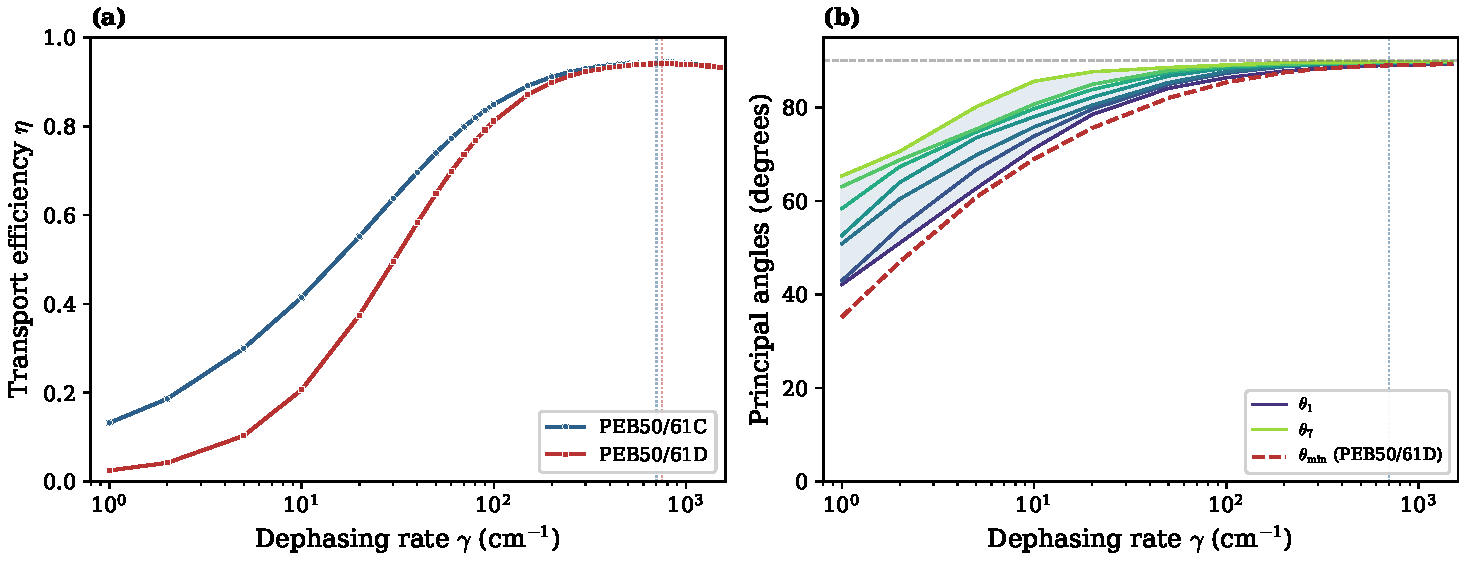
\includegraphics[width=0.92\textwidth]{fig7_pe545.pdf}
\caption{PE545 results.  Same near-classical geometric signature as FMO, despite completely different chromophore types, symmetry, and energy landscape.}
\end{figure}

\subsection*{Neural oscillations ($d = 10$)}

To test where neural systems sit on the quantum-classical spectrum, the paper constructs a $d = 10$ cortical gamma-oscillation assembly (30--70\,Hz, small-world coupling).

\begin{itemize}[leftmargin=1.5em]
\item \textbf{Collapse:} $99 \to 9$ dimensions.
\item \textbf{Biological dephasing:} $\gamma_{\mathrm{bio}}/J_{\max} \approx 8 \times 10^{12}$.
\item \textbf{Geometry at bio dephasing:} All 9 principal angles asymptotically $\to 90^\circ$ (already $>89.5^\circ$ at proxy $\gamma/J_{\max} = 50$).  Deep classical.
\item \textbf{Detection threshold:} ${\sim}14$ orders of magnitude of microenvironment shielding would be needed for any quantum effect to become geometrically distinguishable at oscillation-frequency scales.
\item \textbf{But at molecular scales:} Ion channels ($d \sim 4$) operate at $\gamma_{\mathrm{bio}}/J_{\max} \sim O(1$--$30)$---the same regime as FMO/PE545.  The paper defines a non-classicality index $\chi$ and coordinated dimensionality $D_{\mathrm{coord}}$ to formalize this: deep classical oscillations ($\chi_{\mathrm{osc}} \approx 0$) reliably coordinate $N$ non-classical molecular sites ($\chi_m > 0$), so representational dimensionality scales with $N$, not oscillation frequency.
\item \textbf{Effect-size split:} Absolute uplift scales as $\Delta D_{\mathrm{coord}} = N\chi_m(d_m^2-d_m)$, while relative uplift is fixed at $R_{\mathrm{coord}}=1+\chi_m d_m$ (Fig.~9). For the ion-channel anchor, this is small per site but accumulates with large $N$.
\end{itemize}

\begin{figure}[ht]
\centering
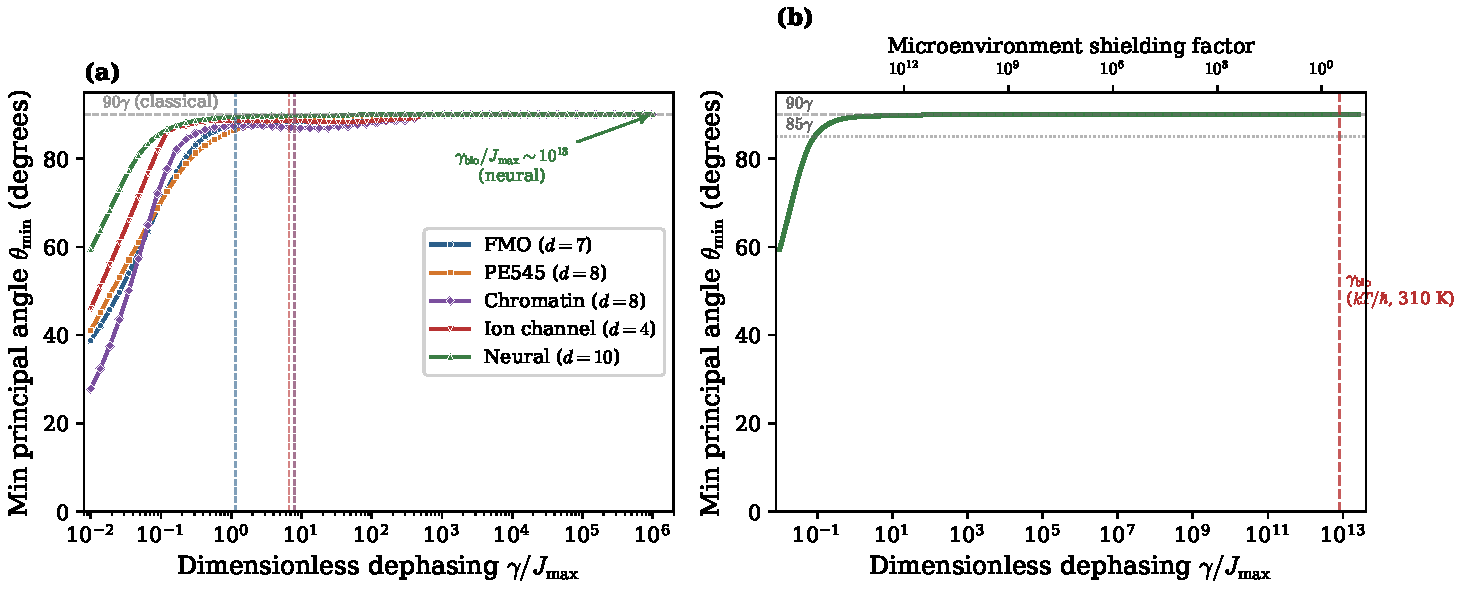
\includegraphics[width=0.92\textwidth]{fig8_neural_comparison.pdf}
\caption{Cross-scale comparison.  Photosynthetic complexes and illustrative molecular models (ion channel, chromatin) sit near the quantum-classical transition; neural oscillations are ${\sim}12$ orders of magnitude past it.  The detection threshold (right) shows how much microenvironment shielding would be needed.}
\end{figure}

An empirical validation using the Potjans--Diesmann cortical column model ($d = 8$) gives the same result, confirming the conclusion is not an artifact of the synthetic Hamiltonian.

\subsection*{The punchline}

Three validated systems spanning $12$ orders of magnitude in dephasing, plus two illustrative molecular models, all follow the same geometric framework: \textbf{photosynthetic and molecular-scale systems sit near the quantum-classical boundary; neural oscillator assemblies are deep classical at oscillation-frequency scales but coordinate molecular systems that remain non-classical ($\chi_m>0$).}

The paper formalizes this as a \textbf{multi-scale architecture}: a non-classicality index $\chi$ (Definition~3.11) measures departure from the classical simplex, and a coordinated dimensionality $D_{\mathrm{coord}}$ (Definition~6.1) shows that effective dimensionality scales with entrained site count $N$, not oscillation frequency.  Proposition~6.3 then separates absolute and relative effect sizes: absolute uplift can accumulate with area, while relative uplift remains locally constrained by $\chi_m$ and $d_m$.

An illustrative ion-channel model ($d = 4$; Appendix~C) gives $\theta_{\min}\approx 88.5^\circ$ and $\chi\approx2.8\times10^{-4}$ at biological dephasing, i.e.\ non-classical but near-classical geometry.  An additional chromatin model ($d = 8$; Appendix~C) sits near the boundary at reference parameters ($\theta_{\min}\approx87^\circ$) but is sensitivity-limited at weak coupling, motivating future work with experimentally determined Hamiltonians.

\section*{Thermodynamic cost}

Coherences store free energy $\Delta F = k_B T \cdot C_r(\rho)$, where $C_r$ is the relative-entropy coherence measure.  Decoherence destroys this free energy irreversibly.

The cost per collapsed dimension vanishes as $\sim \ln d / d^2$ for large $d$: high-dimensional quantum systems lose many dimensions at low thermodynamic cost per dimension.

The paper is careful: this is precise free-energy accounting, not a claim that the destroyed coherence could have been extracted as work in practice.

\section*{What is standard, and what is new?}

\subsection*{Known before this paper}

\begin{itemize}[leftmargin=1.5em]
\item Dephasing kills off-diagonal matrix elements
\item The Bures metric is the natural metric on quantum states
\item On diagonal states, Bures reduces to Fisher--Rao
\item ENAQT: intermediate dephasing enhances photosynthetic transport
\end{itemize}

\subsection*{New in this paper}

\begin{enumerate}[leftmargin=1.5em]
\item \textbf{Exact qubit angle:} Closed-form $\theta_B$ at every full-rank qubit state (Theorem~3.4)
\item \textbf{Global orthogonality theorem:} For $d \geq 3$, Bures-orthogonality $\iff$ diagonal (Theorem~3.6)
\item \textbf{Perturbative cross-Gram:} Explicit formula for departure from orthogonality near the simplex (Theorem~3.7)
\item \textbf{Principal angle framework for ENAQT:} Replacing scalar coherence measures with the full $d{-}1$ angle spectrum
\item \textbf{Near-classical geometry at ENAQT:} Demonstrated in both FMO and PE545
\item \textbf{Cross-scale application:} Neural oscillator assembly ($d = 10$) shown to be ${\sim}12$ orders of magnitude past the quantum-classical boundary; detection threshold quantified
\end{enumerate}

\section*{What the paper does \emph{not} claim}

\begin{itemize}[leftmargin=1.5em]
\item It does not explain \emph{why} nature has this dimensional architecture (that is metaphysical).
\item It does not derive the Born rule (assumed).
\item It does not claim the near-classical geometry is ``universal'' across all photosynthetic complexes (two is suggestive, not conclusive).
\item It does not claim all thermodynamic questions about coherence are settled.
\end{itemize}

\section*{Reading the paper efficiently}

\begin{table}[ht]
\centering
\begin{tabular}{@{}p{0.42\textwidth}p{0.52\textwidth}@{}}
\toprule
\textbf{If you want to\ldots} & \textbf{Read\ldots} \\
\midrule
Understand the core idea & \S1 Introduction + Figure~1 \\
See the mathematical framework & \S2 (QFIM, Bures metric, effective dimensionality) \\
Read the main theorems & \S3: Thm~3.1 (collapse), 3.4 (angle), 3.6 (global orthogonality) \\
See the thermodynamic cost & \S4 (free energy of coherence) \\
See the FMO application & \S5.1--5.5 + Figures~4, 6 \\
See the PE545 second complex & \S5.7 + Figure~7 \\
See the neural application & \S6 + Figure~8 \\
See the cross-scale comparison & \S6.4 + Table in Appendix~D \\
See the chromatin case study & Appendix~C (illustrative model + sensitivity sweep) \\
Compare to scalar coherence measures & \S5.5 (why $d{-}1$ angles $>$ $\ell_1$-norm) \\
Check the numerics & Appendix~A (RK4, SLD, algorithm) \\
See the PE545 Hamiltonian & Appendix~B (full $8\times 8$ matrix) \\
See the neural parameters & Appendix~D (microcircuit models) \\
\bottomrule
\end{tabular}
\end{table}

\begin{table}[ht]
\centering
\begin{tabular}{@{}cp{0.72\textwidth}@{}}
\toprule
\textbf{Equation} & \textbf{What it says} \\
\midrule
(6) & Collapse ratio: $(d{-}1)/(d^2{-}1) = 1/(d{+}1)$ \\
(9)--(10) & Exact Bures separation angle for qubits \\
(14) & Perturbative cross-Gram near the simplex \\
(15) & Lindblad master equation with dephasing + trapping \\
\bottomrule
\end{tabular}
\end{table}

\subsection*{Suggested reading order}

\begin{enumerate}[leftmargin=1.5em]
\item Abstract and introduction
\item Theorem~3.4 (qubit angle) and Theorem~3.6 (global orthogonality)
\item Section~5 biological application (FMO first, then PE545)
\item Section~6 neural oscillations (cross-scale boundary)
\item Discussion (especially \S7.2, cost-benefit interpretation)
\item Appendix~C chromatin case study (if interested in molecular genericity)
\item Return to \S2 and \S3 for full derivations if desired
\end{enumerate}

\subsection*{Repository contents}

\begin{itemize}[leftmargin=1.5em]
\item \texttt{decoherence\_biology.pdf}: the full manuscript (8 figures)
\item \texttt{reader\_guide.pdf}: this note
\item \texttt{figures/}: all publication figures
\item \texttt{code/fmo\_analysis.py}: Lindblad dynamics, transport, geometry
\item \texttt{code/generate\_figures.py}: reproducible code for all figures
\end{itemize}

\vfill

\begin{center}
\small
This guide is intentionally pedagogical.  For precise theorem statements, hypotheses, and proofs, consult the main manuscript.
\end{center}

\end{document}
